\section{TSDF重建算法}

\par Truncated Signed Distance Function(TSDF)是实时三维重建技术的核心组成部分。此方法利用
深度传感器(如 RGB-D 相机)产生的数据来创建且更新 TSDF 模型,为三维重建提供基础。

\par TSDF 被设计为一种稀疏体素网格的数据结构,其中每一个体素都存储了相对于物体表面的有向距离信
息。该有向距离是以传感器的视角进行定义,对于被观察物体的表面,距离为0;对于物体表面的后
方,距离为正;对于物体表面的前方,距离为负,如图\ref{fig:tsdf_example}\cite{tsdf}所示。

\begin{figure}[htb]
	\centering
	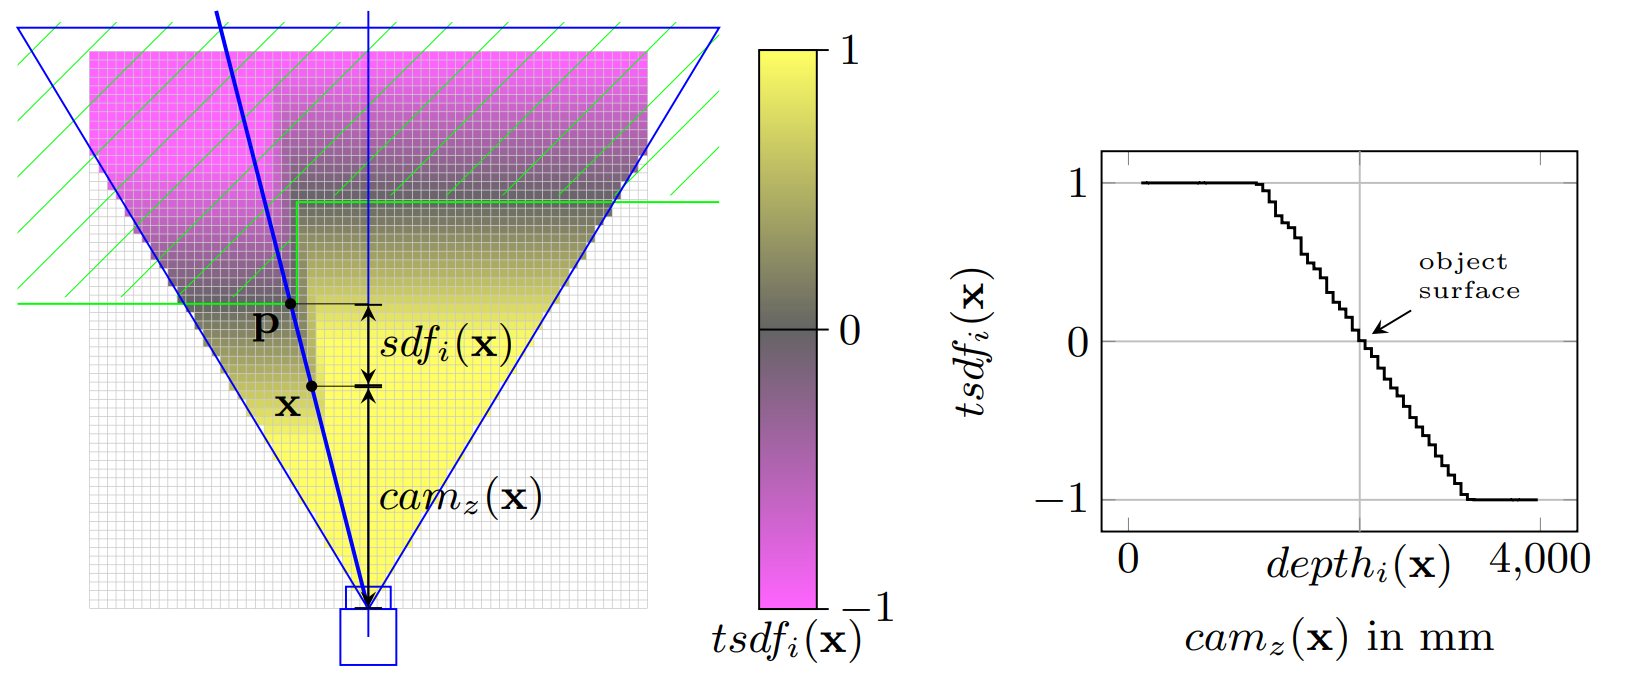
\includegraphics[width=0.9\textwidth]{figures/tsdf_exp.png}
	\caption{TSDF示例}
	\label{fig:tsdf_example}
	\note{注:固体物体:绿色;具有视场、光轴和光线的相机:蓝色;TSDF 网格:看不见的体素为白色,其他体素参见颜色条。体素 x 的有符号距离值由物体表面的深度和体素的相机距离 $cam_z(x)$ 确定。}
\end{figure}

\par 为了生成 TSDF,首先需要从 RGB-D 图像中获得深度信息。对于每一个像素,深度值可以被转
化为一个在三维空间中的点。这些点可以进一步被投影到一个预设的体素网格中,从而生成一个初步
的 TSDF 表示。以下公式描述了该过程:
\begin{equation}
	cam_z(x) = depth_i(pic(x))
\end{equation}
\begin{equation}
	x = K^{-1} pic(x) cam_z(x)
\end{equation}

\par 其中,$x$是世界坐标下的体素点,$pic(x)$是$x$对应的像素坐标,
$cam_z(x)$ 是$x$对应的像素的深度,即该像素所属物体到相机的距离,$K$ 是相机的内参矩阵。

\par 为了获取 TSDF 中每个体素的有向距离,需要计算每个体素中心点到物体表面的最
短距离。在理想情况下,这个距离是物体表面到体素中心的欧氏距离,但是为了方便计算,通常将其
近似为在相机视角下的直线距离。此外,还需要注意距离的截断处理。如果某个体素中心距离
物体表面的距离过大(超过预定的截断距离),则不考虑该体素对 TSDF 的贡献。以下公式描述了该
过程:
\begin{equation}
	sdf_i(x) = depth_i(pic(x)) - cam_z(x)
\end{equation}
\begin{equation}
	tsdf_i(x) = \max(-1, \min(1, \frac{sdf_i(x)}{t}))
\end{equation}

\par 其中,$sdf_i(x)$ 是体素中心点到物体表面的有向距离,$t$ 是预定的截断距离,
$tsdf_i(x)$ 是截断后的 TSDF 距离,$w_{\text{{voxel}}}$ 是体素的权重。

\par 在完成了 TSDF 的初始生成之后,如果输入新的 RGB-D 图像,就需要更新 TSDF。首先,根据相机位姿将新的 RGB-D 图像对齐到当前的 TSDF 模型中,然后
用新图像的数据更新 TSDF 的距离和权重:
\begin{equation}
	TSDF_i(x) = \frac{W_{i-1}(x)TSDF_{i-1}(x) + w_i(x)tsdf_i(x)}{W_{i-1}(x) + w_i(x)}
\end{equation}
\begin{equation}
	W_i(x) = W_{i-1}(x) + w_i(x)
\end{equation}

\par 其中,$W_{i-1}(x)$ 和 $TSDF_{i-1}(x)$ 是旧的 TSDF 体素权重和
距离,$w_i(x)$ 和 $TSDF_i(x)$ 是新的 TSDF 体素权重和距离。

\par TSDF 提供了一种有效的方法从 RGB-D 图像中生成和更新三维重建模型,且具有较好的
噪声抑制和缺失数据填充能力。然而,TSDF 算法也有其局限性,例如无法处理动态场景中的物体运动
,无法处理深度图像中的大范围空洞等。这些问题在后续的研究中也得到了一定程度的解决,例如动
态物体的问题可以通过引入运动分割算法来处理,深度图像中的空洞问题可以通过引入基于RGB图像
的深度补全算法来处理。